\documentclass[12pt, a4paper]{article}
\usepackage{comment}
\usepackage{ragged2e}
\usepackage{amsmath}
\usepackage{xcolor}
\usepackage{multirow}
\usepackage{caption}
\usepackage{tikz}
\usepackage{booktabs}
\usepackage{tabu}
\usepackage{placeins}
\usepackage{pdflscape}
\usetikzlibrary{arrows}
\usepackage{hyperref}
\usepackage{multirow}
\usepackage{subcaption}
 \usepackage{pdflscape}

\captionsetup{font=footnotesize,labelfont=footnotesize}

\hypersetup{
	colorlinks=true,
	linkcolor=blue,
	filecolor=blue,      
	urlcolor=blue,
	citecolor=blue
}

\usepackage{natbib}
\usepackage[title]{appendix}



\def\sym#1{\ifmmode^{#1}\else\(^{#1}\)\fi}


\renewcommand{\today}{\ifcase \month \or January\or February\or March\or %
	April\or May \or June\or July\or August\or September\or October\or November\or %
	December\fi, \number \year} 

\title{Connected Stocks: Evidence from Tehran Stock Exchange}
%\subtitle{}
\author{S.M. Aghajanzadeh\sym{*} \qquad M. Heidari\sym{*} \qquad M. Mohseni\sym{*} \\
	\sym{*} \footnotesize  Tehran Institute for Advanced Studies, Khatam University, Tehran, Iran
}

\def\boxit#1{%
	\smash{\color{red}\fboxrule=1pt\relax\fboxsep=2pt\relax%
		\llap{\rlap{\fbox{\vphantom{0}\makebox[#1]{}}}~}}\ignorespaces
}
\begin{document}
	\maketitle
\section*{Effects}
\subsection*{\textbf{Hypothesis 1}}
 Simple measures of institutional connnectedness statistically and economically improve forecasts of cross-sectional variation in the correlation only for the pairs in the same business group. The effect comes from business group which is the indirect common ownership.

		\begin{table}[htbp]
	\centering
	\caption{text}
	\resizebox{\textwidth}{!}{
		{
\def\sym#1{\ifmmode^{#1}\else\(^{#1}\)\fi}
\begin{tabular}{l*{7}{c}}
\hline\hline
                &\multicolumn{7}{c}{Dependent Variable: Future Monthly Correlation of 4F+Industry Residuals}                                         \\\cmidrule(lr){2-8}
                &\multicolumn{1}{c}{(1)}         &\multicolumn{1}{c}{(2)}         &\multicolumn{1}{c}{(3)}         &\multicolumn{1}{c}{(4)}         &\multicolumn{1}{c}{(5)}         &\multicolumn{1}{c}{(6)}         &\multicolumn{1}{c}{(7)}         \\
\hline
Same Group      &   0.0138\sym{***}&   0.0128\sym{***}&                  &                  &  0.00978\sym{***}&  0.00458         &  0.00356         \\
                &   (5.76)         &   (6.29)         &                  &                  &   (4.29)         &   (1.43)         &   (1.11)         \\
[1em]
$ \text{FCA*} $ &                  &                  &  0.00405\sym{***}&  0.00375\sym{***}&  0.00296\sym{***}&  0.00258\sym{***}&  0.00273\sym{***}\\
                &                  &                  &   (4.94)         &   (5.12)         &   (3.77)         &   (3.53)         &   (3.51)         \\
[1em]
 $ (\text{FCA}^*) \times {\text{SameGroup} }  $ &                  &                  &                  &                  &                  &  0.00524\sym{**} &  0.00517\sym{**} \\
                &                  &                  &                  &                  &                  &   (3.21)         &   (3.18)         \\
\hline
Observations    &   388492         &   388492         &   388492         &   388492         &   388492         &   388492         &   388492         \\
Group Effect    &       No         &       No         &       No         &       No         &       No         &       No         &      Yes         \\
Controls        &       No         &      Yes         &       No         &      Yes         &      Yes         &      Yes         &      Yes         \\
$ R^2 $         & 0.000404         &  0.00200         & 0.000423         &  0.00201         &  0.00229         &  0.00245         &  0.00875         \\
\hline\hline
\multicolumn{8}{l}{\footnotesize \textit{t} statistics in parentheses}\\
\multicolumn{8}{l}{\footnotesize \sym{*} \(p<0.05\), \sym{**} \(p<0.01\), \sym{***} \(p<0.001\)}\\
\end{tabular}
}

	}
\end{table}

	\FloatBarrier
	\newpage
	
\subsection*{\textbf{Hypothesis 2}}
 Pairs of companies belonging to the same business group have a higher correlation than pairs not in the same group. In addition, Pairs that belong to the same group and have a common ownership co-move more than pairs that don't have common ownership. 
 
\begin{landscape}
	\begin{table}[htbp]
		\caption{Non-connected Co-movement}
		\label{AllPairs}
		\resizebox{1.7\textwidth}{!}{
			{
\def\sym#1{\ifmmode^{#1}\else\(^{#1}\)\fi}
\begin{tabular}{l*{7}{c}}
\hline\hline
                &\multicolumn{7}{c}{Dependent Variable: Future Pairs' co-movement}                                                                   \\\cmidrule(lr){2-8}
                &\multicolumn{1}{c}{(1)}         &\multicolumn{1}{c}{(2)}         &\multicolumn{1}{c}{(3)}         &\multicolumn{1}{c}{(4)}         &\multicolumn{1}{c}{(5)}         &\multicolumn{1}{c}{(6)}         &\multicolumn{1}{c}{(7)}         \\
\hline
SameGroup       &   0.0156\sym{***}&                  &   0.0158\sym{***}&                  &                  &   0.0138\sym{***}&   0.0131\sym{***}\\
                &   (9.84)         &                  &  (10.22)         &                  &                  &   (8.27)         &   (7.68)         \\
[1em]
$ \text{MFCAP*}  $&                  &-0.0000723         &-0.000277         &  0.00169         &-0.000322\sym{*}  &-0.000390\sym{**} &-0.000427\sym{*}  \\
                &                  &  (-0.44)         &  (-1.80)         &   (1.42)         &  (-2.19)         &  (-2.70)         &  (-2.29)         \\
[1em]
 $ (\text{MFCAP}^*) \times {\text{SameGroup} }  $ &                  &                  &                  &                  &                  &  0.00313\sym{**} &  0.00364\sym{**} \\
                &                  &                  &                  &                  &                  &   (2.80)         &   (3.34)         \\
\hline
Controls        &      Yes         &      Yes         &      Yes         &      Yes         &      Yes         &      Yes         &      Yes         \\
Sub-Sample      &    Total         &    Total         &    Total         &SameGroups         &   Others         &    Total         &    Total         \\
Business Group FE&       No         &       No         &       No         &       No         &       No         &       No         &      Yes         \\
Observations    &  6018646         &  6018646         &  6018646         &   114526         &  5904120         &  6018646         &  6018646         \\
\hline\hline
\multicolumn{8}{l}{\footnotesize \textit{t} statistics in parentheses}\\
\multicolumn{8}{l}{\footnotesize \sym{*} \(p<0.05\), \sym{**} \(p<0.01\), \sym{***} \(p<0.001\)}\\
\end{tabular}
}

		}
	\end{table}
\end{landscape}

\newpage
\subsection*{\textbf{Hypothesis 3}} 
Stock returns of group affiliated firms exhibit robustly positive comovement even after controlling for both market and industry effects. Group betas
($ \beta_{Businussgroup} $) are highly significant across all models.



			\begin{table}[htbp]
		\centering
		\caption{Cross-sectional average of the time-series coefficients}
		\resizebox{\textwidth}{!}{
			
			{
\def\sym#1{\ifmmode^{#1}\else\(^{#1}\)\fi}
\begin{tabular}{l*{5}{c}}
\hline\hline
                &\multicolumn{5}{c}{ $ \text{Return}\_i - r\_f = R\_i$ }                                          \\\cmidrule(lr){2-6}
                &\multicolumn{1}{c}{(1)}         &\multicolumn{1}{c}{(2)}         &\multicolumn{1}{c}{(3)}         &\multicolumn{1}{c}{(4)}         &\multicolumn{1}{c}{(5)}         \\
\hline
 $ R\_M $        &    0.898\sym{***}&    0.665\sym{***}&    0.728\sym{***}&    0.363\sym{***}&    0.416\sym{***}\\
                &  (39.40)         &  (19.93)         &  (20.74)         &  (12.76)         &  (11.15)         \\
[1em]
 $ R\_{Industry} $ &                  &    0.302\sym{***}&    0.290\sym{***}&    0.184\sym{***}&    0.168\sym{***}\\
                &                  &   (5.88)         &   (5.43)         &   (6.43)         &   (5.64)         \\
[1em]
 $ R\_{Business group} $ &                  &                  &                  &    0.447\sym{***}&    0.453\sym{***}\\
                &                  &                  &                  &  (13.88)         &  (13.91)         \\
[1em]
 $ SMB $        &                  &                  &    0.227\sym{***}&                  &    0.157\sym{***}\\
                &                  &                  &   (8.57)         &                  &   (5.93)         \\
[1em]
 $ UMD $        &                  &                  &   0.0315\sym{*}  &                  & -0.00268         \\
                &                  &                  &   (2.38)         &                  &  (-0.16)         \\
[1em]
 $ HML $        &                  &                  &   0.0106         &                  & 0.000198         \\
                &                  &                  &   (0.53)         &                  &   (0.01)         \\
[1em]
Constant        &    0.204\sym{***}&    0.132\sym{***}&   0.0758\sym{***}&   0.0576\sym{***}&  0.00885         \\
                &   (7.71)         &   (7.27)         &   (4.16)         &   (6.64)         &   (0.67)         \\
\hline
Observations    &   351728         &   351728         &   351728         &   351728         &   351728         \\
\(R^{2}\)       &    0.140         &    0.224         &    0.251         &    0.684         &    0.695         \\
\hline\hline
\multicolumn{6}{l}{\footnotesize \textit{t} statistics in parentheses}\\
\multicolumn{6}{l}{\footnotesize \sym{*} \(p<0.05\), \sym{**} \(p<0.01\), \sym{***} \(p<0.001\)}\\
\end{tabular}
}

		
		}
	\end{table}


\newpage

\section*{Channels} 
\subsection*{Trading}
% 
%For each firm, we calculate daily institutional imbalances, which is the net buying value of institutional investors relative to total traded value on that day ($ \text{InsImb} = \frac{\text{Buy}_{\text{value}} - \text{Sell}_{\text{value}}}{\text{Buy}_{\text{value}} + \text{Sell}_{\text{value}}} $). 
%We expect that institutional imbalances have a lower variation in groups due to the correlated tradings that the ultimate owner ordered to do. So, we calculate the monthly standard deviation of the group's imbalances and compare them to unaffiliated ones. As we expected grouped standard error is  13.1\% and significantly (with t-stat of 12.57) lower than ungrouped firms. 
%
%\begin{table}[htbp]
%	\centering
%	\resizebox{0.75\textwidth}{!}{
%\begin{tabular}{lcccccc}
	\hline\hline
	& \multicolumn{1}{l}{count} & \multicolumn{1}{l}{mean} &
	
	\multicolumn{1}{l}{std} & \multicolumn{1}{l}{min} &
	\multicolumn{1}{l}{median} & \multicolumn{1}{l}{max} \\
	\midrule
	Ungrouped & 60    & 0.645 & 0.063 & 0.492 & 0.653 & 0.784 \\
	\addlinespace
	Grouped & 60    & 0.514 & 0.050 & 0.406 & 0.514 & 0.625 \\
	\hline\hline
\end{tabular}%	
%}
%	\label{tab:addlabel}%
%\end{table}%
%
%
%
%\begin{figure}[htbp]
%	\centering
%	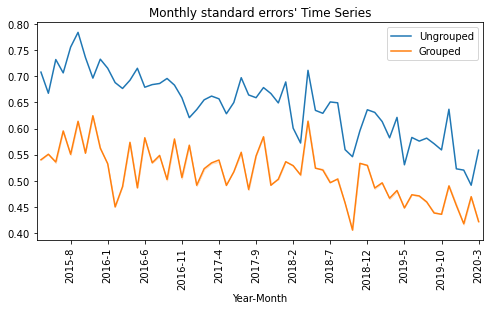
\includegraphics[width=0.8\linewidth]{GroupedSTD}
%	\label{fig:groupedstd}
%\end{figure}
%
%According to the main hypothesis, we need to compare comovement between pairs in groups with low standard error and other pairs.
% For this purpose, we define \textbf{Low Imbalance std} dummy for groups whose average standard errors are lower than half of the sample. 
%So, this dummy is equal to one if at least one pair's firms belong to the low imbalance std business group.
%\begin{table}[htbp]
%	\centering
%	\resizebox{\textwidth}{!}{
%		{
\def\sym#1{\ifmmode^{#1}\else\(^{#1}\)\fi}
\begin{tabular}{l*{6}{c}}
\hline\hline
                    &\multicolumn{6}{c}{Dependent Variable:  Future Pairs's Comovement}                                                                 \\\cmidrule(lr){2-7}
                    &\multicolumn{1}{c}{(1)}         &\multicolumn{1}{c}{(2)}         &\multicolumn{1}{c}{(3)}         &\multicolumn{1}{c}{(4)}         &\multicolumn{1}{c}{(5)}         &\multicolumn{1}{c}{(6)}         \\
\hline
SameGroup           &      0.0208\sym{***}&      0.0206\sym{***}&                     &                     &     0.00619         &     0.00630\sym{*}  \\
                    &      (7.91)         &      (7.94)         &                     &                     &      (1.95)         &      (2.04)         \\
[1em]
LowImbalanceStd     &                     &    -0.00144         &      0.0282\sym{***}&    -0.00724\sym{***}&    -0.00610\sym{***}&    -0.00267         \\
                    &                     &     (-1.15)         &      (6.06)         &     (-5.74)         &     (-4.87)         &     (-1.85)         \\
[1em]
 $ \text{LowImbalanceStd} \times {\text{SameGroup} } $ &                     &                     &                     &                     &      0.0358\sym{***}&      0.0325\sym{***}\\
                    &                     &                     &                     &                     &      (8.57)         &      (7.48)         \\
\hline
Sub-sample          &       Total         &       Total         &   SameGroup         &      Others         &       Total         &       Total         \\
Business Group FE   &          No         &          No         &          No         &          No         &          No         &         Yes         \\
Observations        &      354209         &      354209         &       43274         &      310935         &      354209         &      354209         \\
\hline\hline
\multicolumn{7}{l}{\footnotesize \textit{t} statistics in parentheses}\\
\multicolumn{7}{l}{\footnotesize \sym{*} \(p<0.05\), \sym{**} \(p<0.01\), \sym{***} \(p<0.001\)}\\
\end{tabular}
}

%	}
%\end{table}
%\FloatBarrier

Furthermore, we should show that stocks in groups have a similar daily trading behavior. Accordingly, for each firm we run time-series regressions of the firm's daily change in trading measure, $ \Delta \text{Measure}_{i,t} $, on changes in market measure,$ \Delta\text{Measure}_{Market,t}   $ , changes in the industry and business group portfolio's measure,$ \Delta\text{Measure}_{Ind,t} $ and  $\Delta \text{Measure}_{Group,t} $ and  ,as well as control variables.

 We compute the daily change of measure by this definition $ \Delta \text{Measure}_{i,t} = \ln(\frac{\text{Measure}_{i,t}}{\text{Measure}_{i,t-1}}) $. 
We estimate the following regression for each stock across trading days in given year separately and cross-sectional averages of the estimated coefficients are reported, with t-statistics in parentheses :

\begin{equation*}
	\begin{split}
			\Delta \text{Measure}_{i,t} =  & \text{	}\alpha + \beta_{Market,t} \Delta \text{Measure}_{Market,t}  
		+ \beta_{Ind,t} \Delta \text{Measure}_{Ind,t} \\ & + \beta_{Group,t} \Delta \text{Measure}_{Group,t} + \delta\text{Controls} + \varepsilon_{i,t}
	\end{split}
\end{equation*}

We use the turnover measure as a daily trading measures. We control for lead and lag changes in the two portfolio  and market's measures. In addition, we use size of the firm. [Table \ref{turnover}]

	\begin{table}[htbp]
	\centering
	\caption{cross-sectional average of the time-series coefficients for daily changes in turnover }
	\resizebox{0.7\textheight}{!}{
		{
\def\sym#1{\ifmmode^{#1}\else\(^{#1}\)\fi}
\begin{tabular}{l*{4}{c}}
\hline\hline
                    &\multicolumn{4}{c}{Dependent Variable: $\Delta \text{TurnOver}\_{i} $ }                 \\\cmidrule(lr){2-5}
                    &\multicolumn{1}{c}{(1)}         &\multicolumn{1}{c}{(2)}         &\multicolumn{1}{c}{(3)}         &\multicolumn{1}{c}{(4)}         \\
\hline
 $ \Delta \text{TurnOver}_{\text{Market}} $ &       0.416\sym{***}&       0.326\sym{***}&       0.252\sym{***}&       0.228\sym{***}\\
                    &     (12.25)         &      (5.35)         &      (6.41)         &      (4.24)         \\
[1em]
 $ \Delta \text{TurnOver}_{\text{Industry-i}} $ &       0.142\sym{***}&       0.213\sym{***}&      0.0335         &       0.167\sym{**} \\
                    &      (3.79)         &      (6.29)         &      (1.34)         &      (2.87)         \\
[1em]
 $ \Delta \text{TurnOver}_{\text{Group,-i}} $ &                     &                     &       0.330\sym{***}&       0.218\sym{***}\\
                    &                     &                     &     (12.74)         &      (3.80)         \\
\hline
Control             &          No         &         Yes         &          No         &         Yes         \\
Observations        &      854662         &      851772         &      333789         &      331263         \\
$ R^2 $             &       0.285         &       0.543         &       0.433         &       0.712         \\
\hline\hline
\multicolumn{5}{l}{\footnotesize \textit{t} statistics in parentheses}\\
\multicolumn{5}{l}{\footnotesize \sym{*} \(p<0.05\), \sym{**} \(p<0.01\), \sym{***} \(p<0.001\)}\\
\end{tabular}
}

	} \label{turnover}
\end{table}


%	\begin{table}[htbp]
%	\centering
%	\caption{cross-sectional average of the time-series coefficients for daily changes in illiquidity  }
%	\resizebox{0.7\textheight}{!}{
%		\centering
%		{
\def\sym#1{\ifmmode^{#1}\else\(^{#1}\)\fi}
\begin{tabular}{l*{6}{c}}
\hline\hline
                    &\multicolumn{6}{c}{Dependent Variable: $\Delta \text{Amihud}_{i} $ }                                                               \\\cmidrule(lr){2-7}
                    &\multicolumn{1}{c}{(1)}         &\multicolumn{1}{c}{(2)}         &\multicolumn{1}{c}{(3)}         &\multicolumn{1}{c}{(4)}         &\multicolumn{1}{c}{(5)}         &\multicolumn{1}{c}{(6)}         \\
\hline
 $ \Delta \text{Amihud}_{\text{Market}} $ &       0.324\sym{***}&       0.598\sym{*}  &       0.373\sym{***}&       0.327\sym{***}&       0.391\sym{***}&       0.346\sym{***}\\
                    &      (6.46)         &      (2.17)         &     (13.09)         &     (12.07)         &     (13.09)         &     (12.27)         \\
[1em]
 $ \Delta \text{Amihud}_{\text{Group}} $ &                     &                     &       0.165\sym{**} &       0.150\sym{*}  &       0.143\sym{*}  &       0.126\sym{*}  \\
                    &                     &                     &      (2.60)         &      (2.58)         &      (2.07)         &      (1.98)         \\
[1em]
 $ \Delta \text{Amihud}_{\text{Industry}} $ &      0.0567         &       0.118         &    -0.00390         &    -0.00278         &    -0.00322         &   0.0000345         \\
                    &      (1.21)         &      (1.58)         &     (-0.06)         &     (-0.04)         &     (-0.04)         &      (0.00)         \\
\hline
Observations        &      293264         &      291933         &      184699         &      183301         &      184699         &      183301         \\
Weight              &           -         &           -         & $ \text{MC} \times \text{CR} $          & $ \text{MC} \times \text{CR} $          & $ \text{MC} $          & $ \text{MC} $          \\
Control             &          No         &         Yes         &          No         &         Yes         &          No         &         Yes         \\
$ R^2 $             &      0.0976         &       0.149         &       0.194         &       0.235         &       0.199         &       0.239         \\
\hline\hline
\multicolumn{7}{l}{\footnotesize \textit{t} statistics in parentheses}\\
\multicolumn{7}{l}{\footnotesize \sym{*} \(p<0.05\), \sym{**} \(p<0.01\), \sym{***} \(p<0.001\)}\\
\end{tabular}
}

%	}
%\label{Amihud}
%\end{table}

%In a second test of our proposed channel, we control for stock  characteristics in a multivariate regression. we regress $ \beta_{Group} $
%on the previous year's excess control right from cash flow right, controlling for firm size and average of trading measure. In our main
%specification, we include time-fixed effects and cluster the standard errors at the firm and time-dimension level to account for time-series and cross-sectional dependence. [Table \ref{Turnovercrosssection},\ref{Amihudcrosssection}]  The specification is :
%\begin{equation*}
%	\begin{split}
%		\beta_{Group,i,t} =& \alpha + \beta_1 \text{GroupVariable}_{i,t-1} + \beta_2 \ln(\text{Size})_{i,t-1} \\
%		&+ \beta_3 \text{trading measure}(avg)_{i,t-1} + \text{time effects} + \varepsilon_{i,t-1}
%	\end{split}
%\end{equation*}
%which our group variables are:
%	\begin{enumerate}
%	\item $ \text{Excess} = (\text{cr} - \text{cfr})/\text{cr} $
%	\item $ \text{ExcessDiff} = \text{cr} - \text{cfr} $
%	\item $ \text{ExcessDummy} = \left\{\begin{array}{ll}
%		1 & \text{cr} - \text{cfr}>0\\
%		0 & \text{cr} - \text{cfr}\leq 0
%	\end{array}\right.  $
%	\item $ \text{ExcessHigh} = \left\{\begin{array}{ll}
%		1 & \text{Excess}\geq\text{Q3}(\text{Excess})\\
%		0 & \text{Excess}<\text{Q3}(\text{Excess})
%	\end{array}\right.  $
%\item $ \text{Low Imbalance std} = \left\{\begin{array}{ll}
%	1 & std_{InsImb,t}\leq\text{Median}(std_{InsImb,t})\\
%	0 & std_{InsImb,t}>\text{Median}(std_{InsImb,t})
%\end{array}\right.  $
%
%\end{enumerate}
%
%
%
%	\begin{table}[htbp]
%	\centering
%	\caption{$ \beta_{Group} $ of daily changes in the turnover on Excess control right ($ (cr - cf)/cr $) and other measures   }
%	\resizebox{0.7\textheight}{!}{
%		\centering
%		{
\def\sym#1{\ifmmode^{#1}\else\(^{#1}\)\fi}
\begin{tabular}{l*{14}{c}}
\hline\hline
                &\multicolumn{14}{c}{Dependent Variable: $ \beta\_{Group} $ }                                                                                                                                                                                                              \\\cmidrule(lr){2-15}
                &\multicolumn{1}{c}{(1)}         &\multicolumn{1}{c}{(2)}         &\multicolumn{1}{c}{(3)}         &\multicolumn{1}{c}{(4)}         &\multicolumn{1}{c}{(5)}         &\multicolumn{1}{c}{(6)}         &\multicolumn{1}{c}{(7)}         &\multicolumn{1}{c}{(8)}         &\multicolumn{1}{c}{(9)}         &\multicolumn{1}{c}{(10)}         &\multicolumn{1}{c}{(11)}         &\multicolumn{1}{c}{(12)}         &\multicolumn{1}{c}{(13)}         &\multicolumn{1}{c}{(14)}         \\
\hline
Excess          &    0.355\sym{***}&    0.505\sym{***}&                  &                  &                  &                  &                  &                  &                  &                  &                  &                  &                  &                  \\
                &   (4.99)         &   (6.94)         &                  &                  &                  &                  &                  &                  &                  &                  &                  &                  &                  &                  \\
[1em]
ExcessDummy     &                  &                  &  0.00604         &    0.101\sym{**} &                  &                  &                  &                  &                  &                  &                  &                  &                  &                  \\
                &                  &                  &   (0.16)         &   (2.77)         &                  &                  &                  &                  &                  &                  &                  &                  &                  &                  \\
[1em]
ExcessDiff      &                  &                  &                  &                  &    0.716\sym{***}&    0.961\sym{***}&                  &                  &                  &                  &                  &                  &                  &                  \\
                &                  &                  &                  &                  &   (5.99)         &   (7.77)         &                  &                  &                  &                  &                  &                  &                  &                  \\
[1em]
ExcessHigh      &                  &                  &                  &                  &                  &                  &    0.344\sym{***}&    0.412\sym{***}&                  &                  &                  &                  &                  &                  \\
                &                  &                  &                  &                  &                  &                  &   (6.61)         &   (8.48)         &                  &                  &                  &                  &                  &                  \\
[1em]
Low Imbalance std&                  &                  &                  &                  &                  &                  &                  &                  &  -0.0211         &   -0.144\sym{***}&                  &                  &                  &                  \\
                &                  &                  &                  &                  &                  &                  &                  &                  &  (-0.53)         &  (-3.59)         &                  &                  &                  &                  \\
[1em]
Position        &                  &                  &                  &                  &                  &                  &                  &                  &                  &                  & -0.00268         &   0.0308         &                  &                  \\
                &                  &                  &                  &                  &                  &                  &                  &                  &                  &                  &  (-0.17)         &   (1.94)         &                  &                  \\
[1em]
Centrality      &                  &                  &                  &                  &                  &                  &                  &                  &                  &                  &                  &                  &    0.397\sym{*}  &   -0.153         \\
                &                  &                  &                  &                  &                  &                  &                  &                  &                  &                  &                  &                  &   (2.47)         &  (-1.04)         \\
\hline
Observations    &     1349         &     1349         &     1367         &     1367         &     1349         &     1349         &     1367         &     1367         &     1341         &     1341         &     1349         &     1349         &     1299         &     1299         \\
Time FE         &      Yes         &      Yes         &      Yes         &      Yes         &      Yes         &      Yes         &      Yes         &      Yes         &      Yes         &      Yes         &      Yes         &      Yes         &      Yes         &      Yes         \\
Controls        &       No         &      Yes         &       No         &      Yes         &       No         &      Yes         &       No         &      Yes         &       No         &      Yes         &       No         &      Yes         &       No         &      Yes         \\
$ R^2 $         &   0.0251         &   0.0970         & 0.000973         &   0.0600         &   0.0436         &    0.123         &   0.0436         &    0.109         &  0.00130         &   0.0640         &  0.00128         &   0.0581         &  0.00415         &   0.0456         \\
\hline\hline
\multicolumn{15}{l}{\footnotesize \textit{t} statistics in parentheses}\\
\multicolumn{15}{l}{\footnotesize \sym{*} \(p<0.05\), \sym{**} \(p<0.01\), \sym{***} \(p<0.001\)}\\
\end{tabular}
}

%	}
%\label{Turnovercrosssection}
%\end{table}
%
%
%	\begin{table}[htbp]
%	\centering
%	\caption{$ \beta_{Group} $ of daily changes in the Amihud measure  on Excess control right ($ (cr - cf)/cr $) and other measures   }
%	\resizebox{0.7\textheight}{!}{
%		\centering
%		{
\def\sym#1{\ifmmode^{#1}\else\(^{#1}\)\fi}
\begin{tabular}{l*{8}{c}}
\hline\hline
                &\multicolumn{8}{c}{Dependent Variable: $ \beta\_{Group} $ }                                                                                             \\\cmidrule(lr){2-9}
                &\multicolumn{1}{c}{(1)}         &\multicolumn{1}{c}{(2)}         &\multicolumn{1}{c}{(3)}         &\multicolumn{1}{c}{(4)}         &\multicolumn{1}{c}{(5)}         &\multicolumn{1}{c}{(6)}         &\multicolumn{1}{c}{(7)}         &\multicolumn{1}{c}{(8)}         \\
\hline
Excess          &    0.232\sym{**} &    0.403\sym{***}&                  &                  &                  &                  &                  &                  \\
                &   (3.11)         &   (4.12)         &                  &                  &                  &                  &                  &                  \\
[1em]
ExcessDummy     &                  &                  &  -0.0327         &   0.0544         &                  &                  &                  &                  \\
                &                  &                  &  (-0.61)         &   (0.89)         &                  &                  &                  &                  \\
[1em]
ExcessDiff      &                  &                  &                  &                  &    0.399\sym{***}&    0.650\sym{***}&                  &                  \\
                &                  &                  &                  &                  &   (3.31)         &   (4.35)         &                  &                  \\
[1em]
ExcessHigh      &                  &                  &                  &                  &                  &                  &    0.278\sym{***}&    0.369\sym{***}\\
                &                  &                  &                  &                  &                  &                  &   (5.96)         &   (6.74)         \\
\hline
Observations    &     1349         &     1349         &     1367         &     1367         &     1349         &     1349         &     1367         &     1367         \\
Time FE         &      Yes         &      Yes         &      Yes         &      Yes         &      Yes         &      Yes         &      Yes         &      Yes         \\
Controls        &       No         &      Yes         &       No         &      Yes         &       No         &      Yes         &       No         &      Yes         \\
$ R^2 $         &   0.0115         &   0.0551         &  0.00401         &   0.0359         &   0.0138         &   0.0586         &   0.0252         &   0.0694         \\
\hline\hline
\multicolumn{9}{l}{\footnotesize \textit{t} statistics in parentheses}\\
\multicolumn{9}{l}{\footnotesize \sym{*} \(p<0.05\), \sym{**} \(p<0.01\), \sym{***} \(p<0.001\)}\\
\end{tabular}
}

%	}
%\label{Amihudcrosssection}
%\end{table}

\begin{table}[htbp]
	\centering
	\caption{Pairwise correlation in turnover  }
	\resizebox{0.7\textheight}{!}{
		\centering
		{
\def\sym#1{\ifmmode^{#1}\else\(^{#1}\)\fi}
\begin{tabular}{l*{7}{c}}
\hline\hline
                    &\multicolumn{7}{c}{Dependent Variable:  Monthly Correlation of Delta turnover}                                                                           \\\cmidrule(lr){2-8}
                    &\multicolumn{1}{c}{(1)}         &\multicolumn{1}{c}{(2)}         &\multicolumn{1}{c}{(3)}         &\multicolumn{1}{c}{(4)}         &\multicolumn{1}{c}{(5)}         &\multicolumn{1}{c}{(6)}         &\multicolumn{1}{c}{(7)}         \\
\hline
SameGroup           &      0.0180\sym{***}&                     &      0.0173\sym{***}&                     &                     &      0.0150\sym{***}&      0.0168\sym{***}\\
                    &      (6.19)         &                     &      (5.53)         &                     &                     &      (4.89)         &      (5.40)         \\
[1em]
$ \text{MFCAP*} $   &                     &     0.00219\sym{**} &    0.000543         &     0.00115         &    0.000372         &    0.000363         &   -0.000413         \\
                    &                     &      (2.84)         &      (0.69)         &      (0.57)         &      (0.41)         &      (0.40)         &     (-0.37)         \\
[1em]
 $ (\text{MFCAP}^*) \times {\text{SameGroup} }  $ &                     &                     &                     &                     &                     &     0.00260         &     0.00296         \\
                    &                     &                     &                     &                     &                     &      (1.03)         &      (1.19)         \\
\hline
Sub-sample          &         All         &         All         &         All         &   SameGroup         &      Others         &         All         &         All         \\
Business Group FE   &          No         &          No         &          No         &          No         &          No         &          No         &         Yes         \\
Observations        &      294864         &      294864         &      294864         &       37076         &      257788         &      294864         &      294864         \\
\hline\hline
\multicolumn{8}{l}{\footnotesize \textit{t} statistics in parentheses}\\
\multicolumn{8}{l}{\footnotesize \sym{*} \(p<0.05\), \sym{**} \(p<0.01\), \sym{***} \(p<0.001\)}\\
\end{tabular}
}

	}
	\label{mresult2-turnover}
\end{table}

%\begin{table}[htbp]
%	\centering
%	\caption{Pairwise correlations in liquidity}
%	\resizebox{0.7\textheight}{!}{
%		\centering
%		{
\def\sym#1{\ifmmode^{#1}\else\(^{#1}\)\fi}
\begin{tabular}{l*{9}{c}}
\hline\hline
                &\multicolumn{9}{c}{Dependent Variable: Future Monthly Correlation of Delta Amihud}                                                                                        \\\cmidrule(lr){2-10}
                &\multicolumn{1}{c}{(1)}         &\multicolumn{1}{c}{(2)}         &\multicolumn{1}{c}{(3)}         &\multicolumn{1}{c}{(4)}         &\multicolumn{1}{c}{(5)}         &\multicolumn{1}{c}{(6)}         &\multicolumn{1}{c}{(7)}         &\multicolumn{1}{c}{(8)}         &\multicolumn{1}{c}{(9)}         \\
\hline
Same Group      &   0.0116\sym{**} & -0.00482         &                  &                  &  0.00482         & -0.00853\sym{*}  &   0.0103         & -0.00595         & -0.00739         \\
                &   (2.76)         &  (-1.64)         &                  &                  &   (1.17)         &  (-2.49)         &   (1.89)         &  (-1.32)         &  (-1.85)         \\
[1em]
$ \text{FCA*} $ &                  &                  &  0.00650\sym{***}&  0.00303\sym{***}&  0.00585\sym{***}&  0.00363\sym{***}&  0.00634\sym{***}&  0.00384\sym{***}&  0.00289\sym{**} \\
                &                  &                  &   (6.09)         &   (4.52)         &   (6.03)         &   (4.31)         &   (6.04)         &   (4.26)         &   (2.89)         \\
[1em]
 $ (\text{FCA}^*) \times {\text{SameGroup} }  $ &                  &                  &                  &                  &                  &                  & -0.00586\sym{*}  & -0.00274         & -0.00162         \\
                &                  &                  &                  &                  &                  &                  &  (-2.42)         &  (-1.10)         &  (-0.70)         \\
\hline
Observations    &   377863         &   369768         &   377863         &   369768         &   377863         &   369768         &   377863         &   369768         &   369768         \\
Group Effect    &       No         &       No         &       No         &       No         &       No         &       No         &       No         &       No         &      Yes         \\
Controls        &       No         &      Yes         &       No         &      Yes         &       No         &      Yes         &       No         &      Yes         &      Yes         \\
$ R^2 $         & 0.000586         &  0.00615         & 0.000681         &  0.00610         &  0.00117         &  0.00654         &  0.00136         &  0.00673         &   0.0220         \\
\hline\hline
\multicolumn{10}{l}{\footnotesize \textit{t} statistics in parentheses}\\
\multicolumn{10}{l}{\footnotesize \sym{*} \(p<0.05\), \sym{**} \(p<0.01\), \sym{***} \(p<0.001\)}\\
\end{tabular}
}

%	}
%	\label{mresult2-liquidity}
%	\end{table}



\newpage
		\begin{figure}
	\centering  
	\caption{Time series of average common ownership measure with 95 percent interval for all pairs}
	\includegraphics[width=\linewidth]{"FCAtimeSeries.eps"}
	
\end{figure} 

			\begin{figure}
	\centering  
	\caption{Time series of average common ownership measure with 95 percent interval in pairs in the same business group and others}
	\includegraphics[width=\linewidth]{"FCAtimeSeriesBG.eps"}
\end{figure}    

\begin{figure}
	\centering  
	\caption{Time series of average common ownership measure with 95 percent interval which is grouped based on pairs' size}
	\includegraphics[width=\linewidth]{"FCAtimeSeriesPairType.eps"}
\end{figure}




	\begin{figure}
	\centering  
	\caption{Percent of group affiliated firms from listed firms}
	\includegraphics[width=\linewidth]{"BGtimeSeries.eps"}
	
\end{figure}  

\begin{figure}
	\centering  
	\caption{Percent of group affiliated firms from marketcap}
	\includegraphics[width=\linewidth]{"BGMarketCaptimeSeries.eps"}
	
\end{figure}
 
%\begin{figure}
%	\centering  
%	\includegraphics[width=\linewidth]{"CorrtimeSeries.eps"}
%\end{figure}    
%
%\begin{figure}
%	\centering  
%	\includegraphics[width=\linewidth]{"BGCorrtimeSeries.eps"}
%\end{figure}
\end{document}